\documentclass{article}
\usepackage{nirav-ds203}

\newcommand{\myname}{Nirav Bhattad}
\newcommand{\topicname}{DS203 : Exercise 1}

\begin{document}

\thispagestyle{empty}

\titleBC

\section{Part-A (Simple Linear Regression Derivation)}

\subsection{Introduction}

We will derive the formula for simple linear regression. We will use the following notation:

\begin{itemize}
	\item $X$ is the dependent variable.
	\item $Y$ is the independent variable.
	\item $n$ is the number of data points.
	\item $(x_i, y_i)$ is the $i^{th}$ data point.
	\item $\overline{x}$ is the mean of $X$.
	\item $\overline{y}$ is the mean of $Y$.
	\item $\overline{xy}$ is the mean of $XY$.
	\item $\overline{x^2}$ is the mean of $X^2$.
	\item $\overline{y^2}$ is the mean of $Y^2$.
\end{itemize}

\subsection{Derivation}

The formula for the line of best fit is given by:

\begin{align}
	y = ax + b
\end{align}

where $a$ is the slope and $b$ is the intercept. We can derive the formula for $a$ and $b$ by minimizing the sum of squared errors. The sum of squared errors is given by:

\begin{align}
	\sum_{i=1}^{n} (y_i - (ax_i + b))^2
\end{align}

We can minimize this expression by taking the partial derivatives with respect to $a$ and $b$ and setting them to zero. The partial derivative with respect to $a$ is given by:

\begin{align}
	\frac{\partial}{\partial a} \sum_{i=1}^{n} (y_i - (ax_i + b))^2
\end{align}

The partial derivative with respect to $b$ is given by:

\begin{align}
	\frac{\partial}{\partial b} \sum_{i=1}^{n} (y_i - (ax_i + b))^2
\end{align}

Setting these partial derivatives to zero gives us the following two equations:

\begin{align}
	\sum_{i=1}^{n} (y_i - (ax_i + b))x_i &= 0 \\
	\sum_{i=1}^{n} (y_i - (ax_i + b)) &= 0
\end{align}

Solving these equations gives us the following formulas for $a$ and $b$:

\begin{align}
	a &= \dfrac{\overline{xy} - \overline{x} \, \overline{y}}{\overline{x^2} - \overline{x}^2} \\
	b &= \dfrac{\overline{y} \, \overline{x^2} - \overline{x} \, \overline{xy}}{\overline{x^2} - \overline{x}^2}
\end{align}

\subsection{Conclusion}

We have derived the formula for simple linear regression. The equations for slope and intercept are given by:

\begin{align}
	a &= \dfrac{\overline{xy} - \overline{x} \, \overline{y}}{\overline{x^2} - \overline{x}^2} \\
	b &= \dfrac{\overline{y} \, \overline{x^2} - \overline{x} \, \overline{xy}}{\overline{x^2} - \overline{x}^2}
\end{align}

\clearpage



\section{Part-B}

\begin{custombox}[label={box:step1}]{Step 1}
	Using a spreadsheet create a dataset comprising $100$ pairs $(x_i, y_i)$ as per the following guidelines:

	\begin{itemize}
		\item Create $100$ random values of $x_i$ lying between $0$ and $1$ (both inclusive)
		\item Corresponding to each $x_i$, create $y_i$ such that the scatter plot of $y_i$ \textit{v/s} $x_i$ looks like the following:
	\end{itemize}

	\begin{figure}[H]
		\centering
		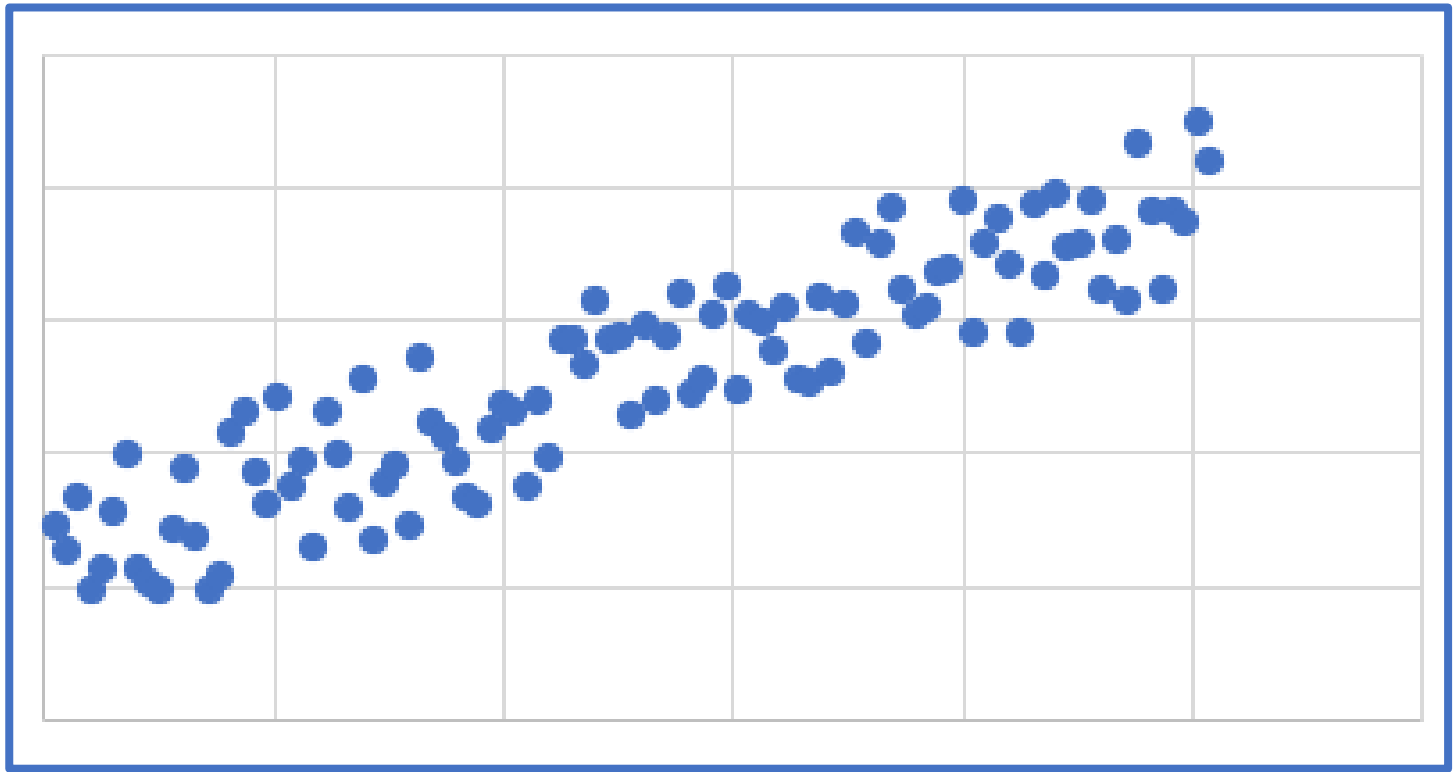
\includegraphics[width=0.5\textwidth]{Images/Step1.png}
		\caption{Randomized Dataset}
	\end{figure}
\end{custombox}

Here, I choose to create a dataset with $100$ random values of $x_i$ between $0$ and $1$ (both inclusive). The corresponding $y_i$ values were calculated using the following formula:

\begin{align}
	y_i = 2 \times x_i + 1 + (\texttt{RAND()} - 0.5) \times 0.4
\end{align}


\begin{custombox}[label={box:step2}]{Step 2}
	Create the scatter plot resulting from your dataset $(x_i, y_i)$
\end{custombox}

\begin{figure}[H]
	\centering
	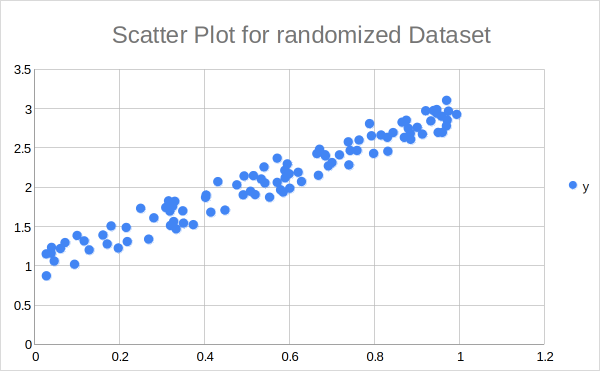
\includegraphics[width=0.5\textwidth]{Images/Step2.png}
	\caption{Scatter Plot for our Dataset}
\end{figure}

\begin{custombox}[label={box:step3}]{Step 3}
	Using the $(x_i, y_i)$ data, calculate the regression coefficients $a$ and $b$ (all calculations should be entirely done using the spreadsheet). The equation of the resulting regression model (line) will be as shown below.

	\begin{align}
		\widehat{y_i} = {a} \cdot {x_i} + b
	\end{align}
\end{custombox}

\begin{figure}[H]
	\centering
	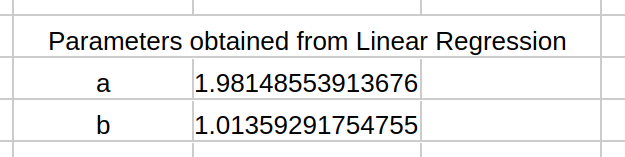
\includegraphics[width=0.5\textwidth]{Images/Step3.png}
	\caption{Regression Coefficients}
\end{figure}

\begin{custombox}[label={box:step4and5}]{Step 4 and Step 5}
	Using this regression line predict $\widehat{y_i}$ corresponding to every $x_i$. Superimpose the regression line over the scatter plot created in Step \ref{box:step3}, as shown below.

	\begin{figure}[H]
		\centering
		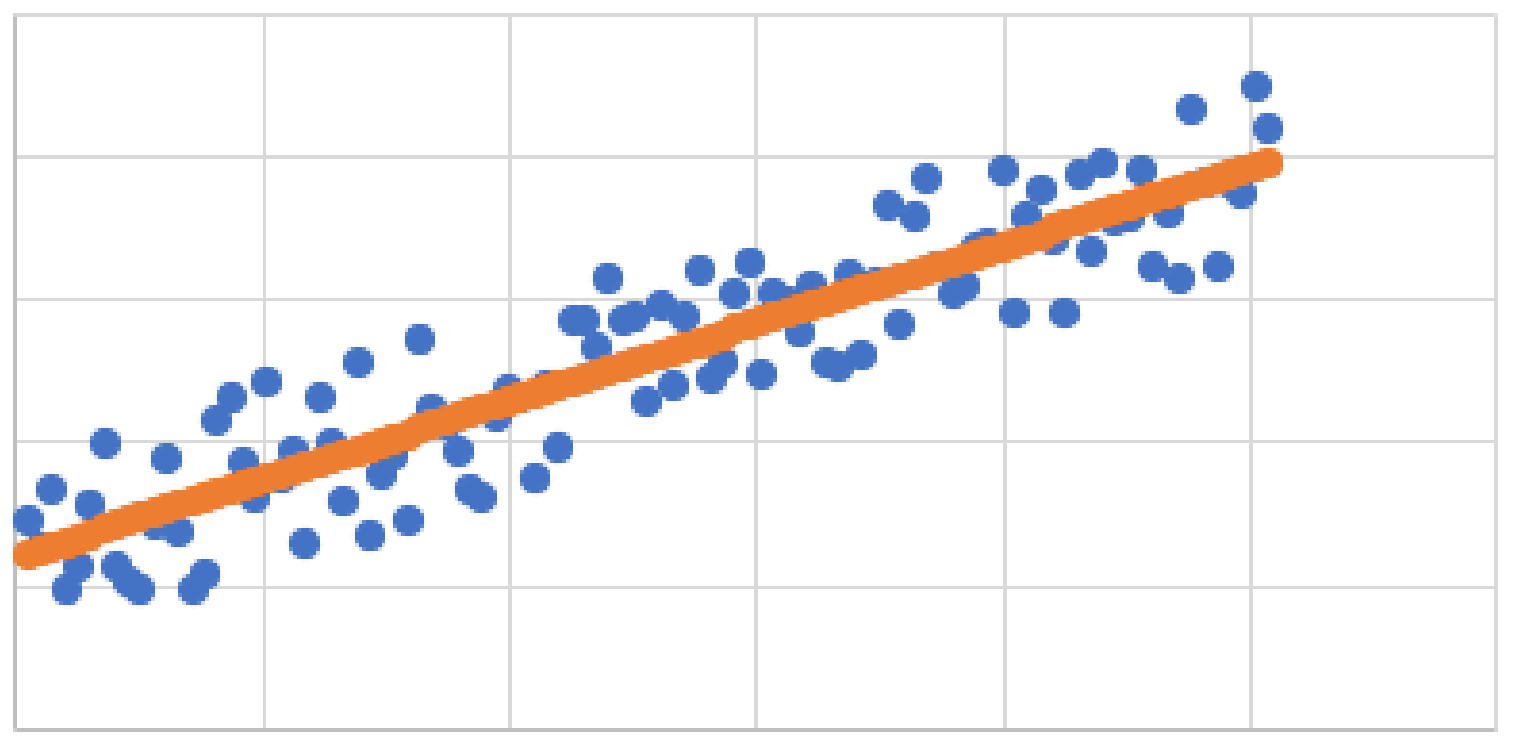
\includegraphics[width=0.5\textwidth]{Images/Step45.png}
		\caption{Regression Line Superimposed on the Scatter Plot}
	\end{figure}
\end{custombox}

\begin{figure}[H]
	\centering
	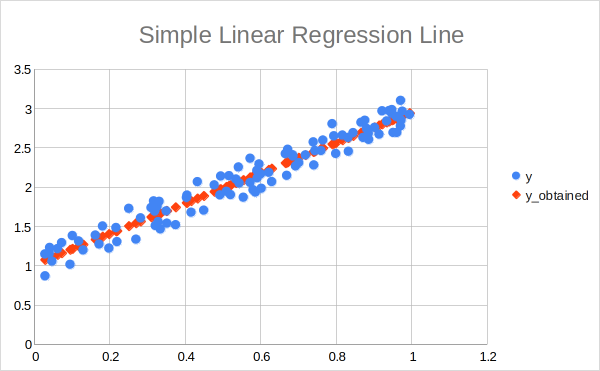
\includegraphics[width=0.5\textwidth]{Images/regression.png}
	\caption{Regression Line Superimposed on the Scatter Plot for my dataset}
\end{figure}

\begin{custombox}[label={box:step6}]{Step 6}
	Calculate the prediction error $e_i$ corresponding to every $y_i$, and calculate the error metrics Sum of Squared Errors (SSE) and Mean Absolute Error (MAE).
\end{custombox}

\begin{figure}[H]
	\centering
	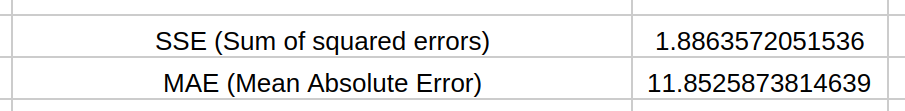
\includegraphics[width=0.5\textwidth]{Images/Step6.png}
	\caption{Error Metrics}
\end{figure}

\begin{custombox}[label={box:step7}]{Step 7}
	Create a scatter plot of $e_i$ v/s $x_i$.
\end{custombox}

\begin{figure}[H]
	\centering
	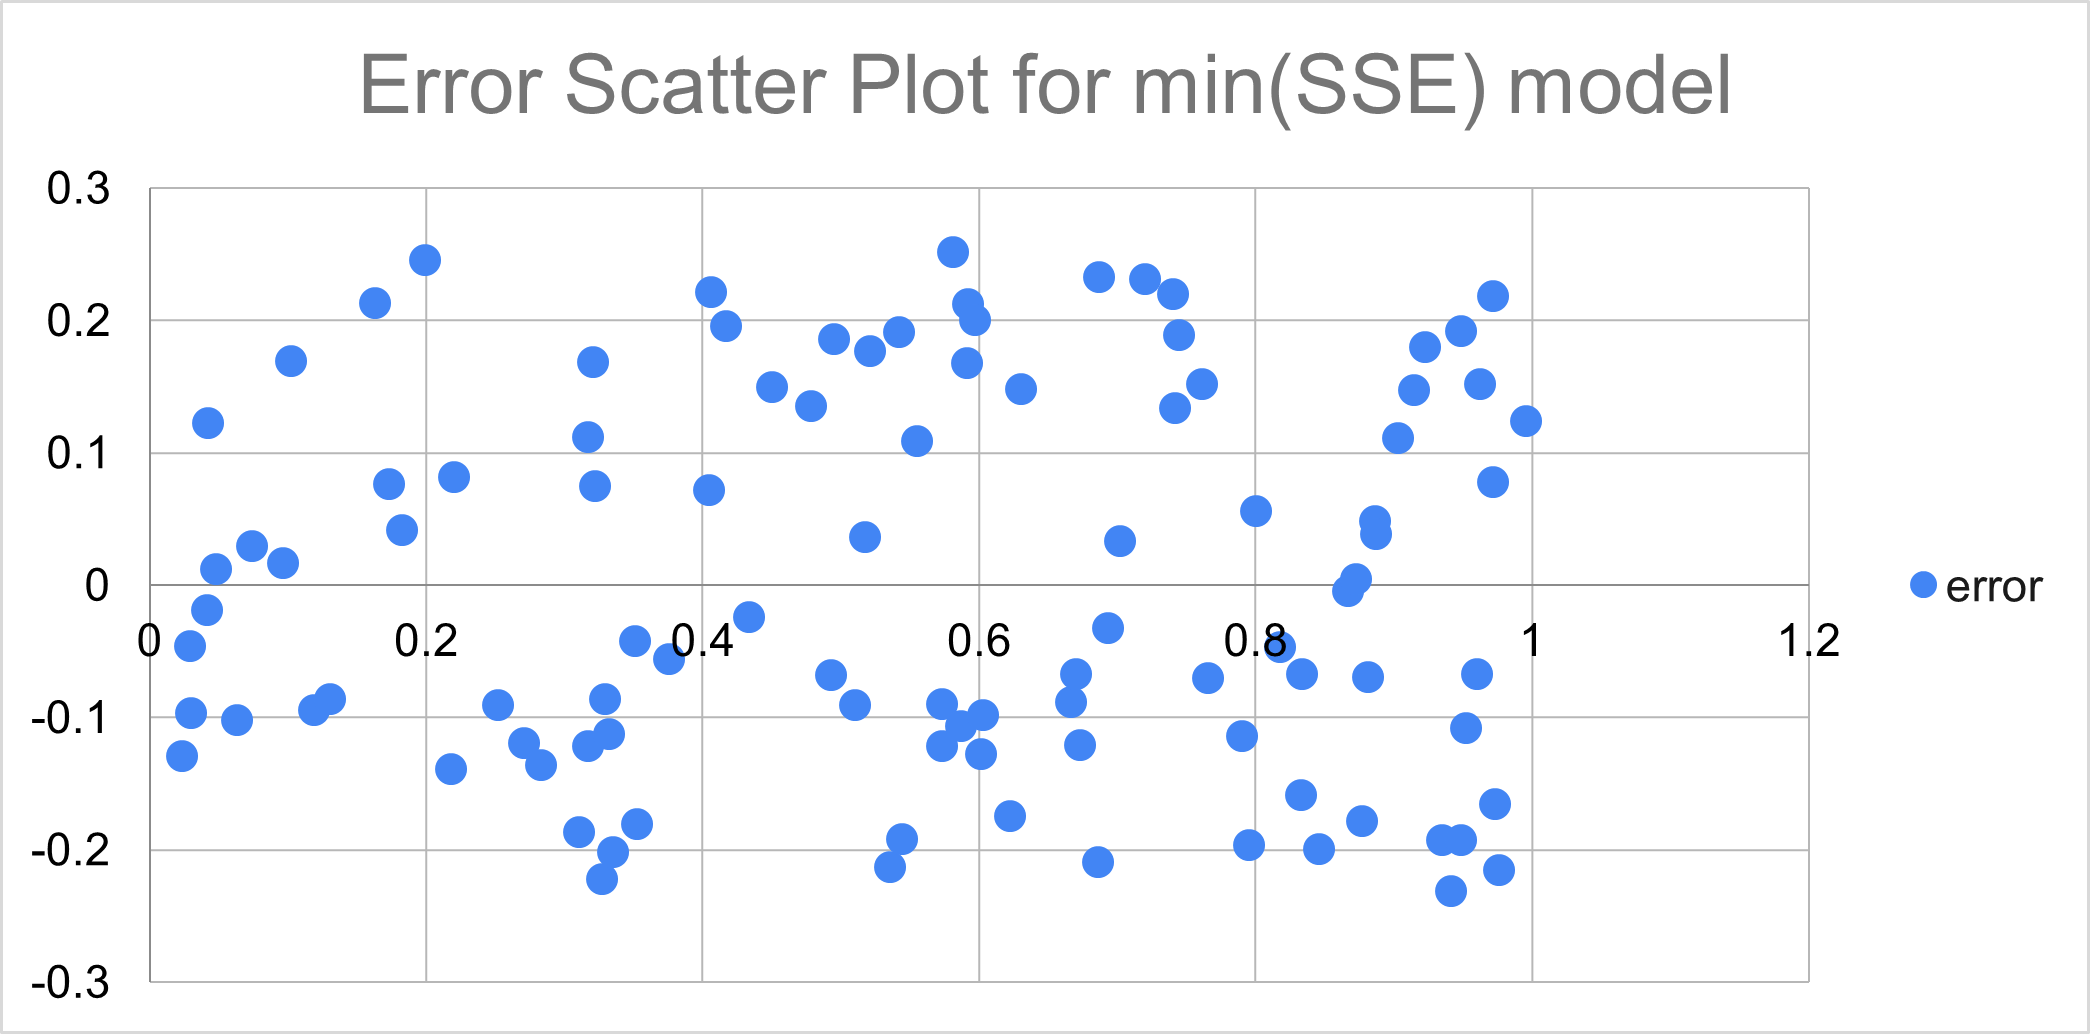
\includegraphics[width=0.5\textwidth]{Images/error1.png}
	\caption{Scatter Plot of $e_i$ \textit{v/s} $x_i$}
\end{figure}

\begin{custombox}[label={box:step8}] {Step 8}
	As discussed in class, the simplest (and na\"{\i}ve) model is one that predicts the mean, as shown below. Using this model calculate $e_i$, SSE and MAE and create the scatter plot of $e_i$ \textit{v/s} $x_i$.

	\begin{align}
		\widehat{y_i} = \overline{y}
	\end{align}
\end{custombox}

\begin{figure}[H]
	\centering
	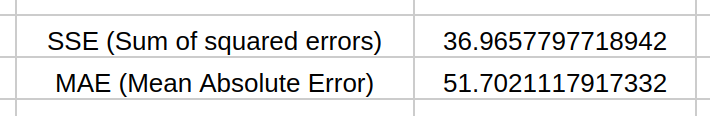
\includegraphics[width=0.5\textwidth]{Images/Step8.png}
	\caption{Scatter Plot of $e_i$ \textit{v/s} $x_i$ for Na\"{\i}ve Model}
	\caption{Error Metrics for Na\"{\i}ve Model}
\end{figure}

\begin{figure}[H]
	\centering
	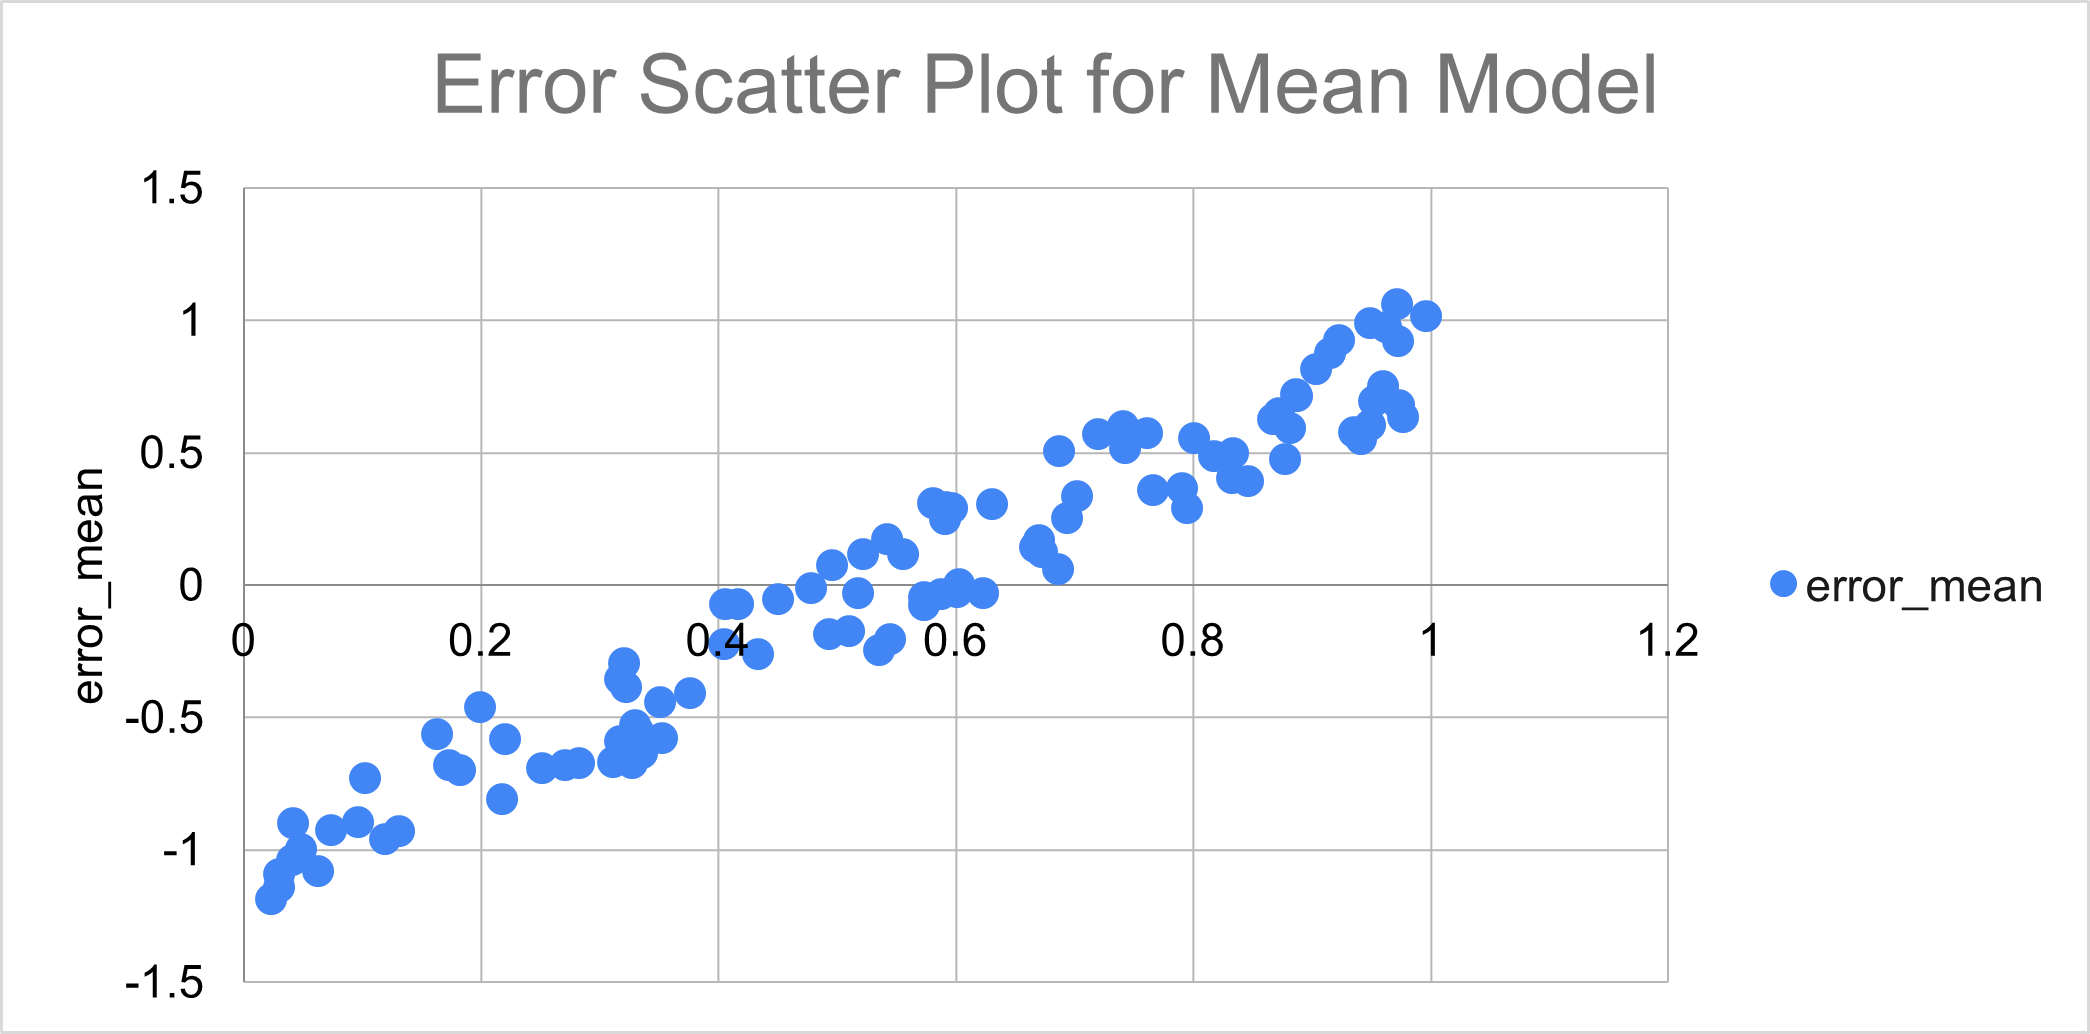
\includegraphics[width=0.5\textwidth]{Images/error2.png}
	\caption{Scatter Plot of $e_i$ \textit{v/s} $x_i$ for Na\"{\i}ve Model}
\end{figure}

\begin{custombox}[label={box:step9}] {Step 9}
	Compare the error metrics and error scatter plots resulting from the above two distinct models and record your analysis and explain the differences between the two error scatter plots. (Note: Stating obvious facts is NOT analysis!)
\end{custombox}

\setcounter{subsection}{9}

\subsubsection{Error Metrics}

\begin{enumerate}
	\item \textbf{Minimum SSE Model:} This model is optimized to minimize the Sum of Squared Errors (SSE). Hence in general we observe a lower SSE and Mean Absolute Error (MAE) value as compared to the Na\"{\i}ve Model, because the model's parameters are specifically adjusted to fit the training data as closely as possible.
	\item \textbf{Mean Model:} This model is a simple model that predicts the mean value of the target variable for all inputs. This model is not optimized for any specific metric, and hence we observe a higher SSE and MAE value as compared to the Minimum SSE Model.
\end{enumerate}

\subsubsection{Error Scatter Plots}

\begin{enumerate}
	\item \textbf{Minimum SSE Model:} The error scatter plot for the Minimum SSE Model shows a random distribution of errors around the $y = 0$ line. This indicates that the model is able to predict the target variable with a certain degree of accuracy, and the errors are distributed randomly around the regression line with almost equal probability to be positive or negative.
	\item \textbf{Mean Model:} The error scatter plot for the Mean Model shows a systematic distribution of errors around the $x = 0.5$ line. This indicates that the model is not able to predict the target variable accurately, and the errors are systematically biased towards one side of the regression line till $x$ is around $0.5$ and then flips signs. In this case, the errors are consistently negative for $x < 0.5$ and consistently positive for $x > 0.5$. The error scatter plot looks almost like a straight line with a slope equal to the slope of the regression line.
\end{enumerate}

\clearpage

\subsubsection{Analysis}

The analysis of the error metrics and error scatter plots for the two models is as follows:

\begin{enumerate}
	\item The Minimum SSE Model is able to predict the target variable more accurately as compared to the Mean Model, as indicated by the lower SSE and MAE values.
	\item The error scatter plot for the Minimum SSE Model shows a random distribution of errors around the regression line, indicating that the model is able to predict the target variable with a certain degree of accuracy.
	\item The error scatter plot for the Mean Model shows a systematic distribution of errors around the $x = 0.5$ line, indicating that the model is not able to predict the target variable accurately and the errors are systematically biased towards one side of the regression line.
	\item The Mean Model is a simple model that predicts the mean value of the target variable for all inputs. This model is not optimized for any specific metric, and hence the errors are systematically biased towards one side of the regression line.
	\item The Minimum SSE Model is optimized to minimize the Sum of Squared Errors (SSE) and hence is able to predict the target variable more accurately as compared to the Mean Model.
	\item The error scatter plot for the Minimum SSE Model shows a random distribution of errors around the regression line, indicating that the model is able to predict the target variable with a certain degree of accuracy.
\end{enumerate}

The main distinction between the error scatter plots of the two models is that the minimum sum of squared errors (SSE) model typically shows a better fit, with residuals spread out randomly around zero, indicating a well-fitted model. In contrast, the residuals of the mean model are more likely to exhibit identifiable patterns, highlighting its failure to accurately capture the nuances of the data. The minimum SSE model's ability to more closely match the data generally leads to significantly improved error metrics, underscoring the effectiveness of model-specific optimization compared to simple average predictions. Finally, we can conclude that the minimum SSE model is more effective in predicting the target variable, as evidenced by its lower error metrics and more evenly distributed residuals.




\section{Main Learnings}

This exercise helped me understand Simple Linear Regression by working directly with it. I created a set of data and determined the values for $a$ and $b$ in the simple linear regression equation. By making a scatter plot and drawing the regression line, I was able to visualize how well the model fits the data. I also calculated prediction errors and used metrics like SSE (Sum of Squared Errors) and MAE (Mean Absolute Error) to assess the model's accuracy. \\

Comparing these metrics with those from a basic model (which just predicts the average) showed why using a regression model is better. This exercise helped me understand why it's important to visualize and analyze errors to understand how well the model is doing and find areas where it can be improved. In the end, I saw a practical demonstration of how theoretical regression analysis connects to real-world use, using tools like spreadsheets.

\end{document}